
\section{Introduction and Description of the Work}

\subsection{Motivation}

Physics simulation is one of the key components of a modern game engine. The more accurate the simulation is, the more immersive any games built with the engine are likely to be. If the world around the player does not react as expected then it is difficult to become immersed in the game environment.

\subsection{Problem}

Most game engines simulate the world using a mesh and rigid body representation. This limits how accurate physical reactions, such as collisions, can be regarding object damage. If two rigid bodies collide then their vector components can be resolved based on their speeds and angles of incidence amongst other properties. However computing the damage to their bodies is less trivial, the meshes can be dented and predetermined joints broken but this leads to objects appearing to lose mass. Damage can look predetermined and independent of the actual collision. As meshes are hollow representations of objects, any calculations involving mass are difficult.

\subsection{Solution}

Representing objects volumetrically allows for more accurate object destruction. Any fragments which would be severed from an object should consist of a portion of that object's mass. If the object is represented as voxels then this can be simulated by breaking voxels from the parent object. Computing the physical properties of the fragments dynamically can then be done based on the number and orientation of voxels they contain\cite{AfD}.

Permanently representing every object volumetrically would become inefficient in scenes with many objects. Instead objects will be represented with meshes and converted to volumes in real-time on collision\cite{RTC}

For example, if a bullet is fired at a brick wall, both the bullet and wall will be rigid meshes when the bullet is shot. On collision, both the wall and bullet will be voxelised. Assuming the bullet consists of only one voxel, no destruction calculations will be performed on it. Using the force of impact and physical parameters of the wall, it will be calculated which voxels should break off. These voxels will then be transformed back into rigid meshes and the correct movement vectors will be applied. The wall's mesh will be reformed based on the new volumetric structure. This is illustrated in figure \ref{fig}.

\begin{figure}

\label{fig}
\centerline{\includegraphics[scale=0.5]{diagram.pdf}}
\caption{A simple rigid mesh projectile is fired towards another rigid mesh (a). On collision a portion of each body is voxelised (b) depending on the force of the projectile and physical parameters of the objects. It is determined which voxels will detach, shown in red. Meshes are reformed around all separate bodies and physical forces are applied (c).}
\end{figure}

\begin{comment}

Current trends in digital gaming are towards sandbox titles, where the player is encouraged to shape and manipulate the world, often by placing and breaking blocks\footnote{See \href{https://minecraft.net/}{Minecraft} by \href{http://mojang.com/}{Mojang}}. This is achieved by storing the state of the world as a three dimensional array of block identifiers, usually batched into `chunks' which are loaded and unloaded as the player approaches them. While this approach has been optimised for memory and CPU load, it presents several limitations with regards to player experience. Players are confined to placing and breaking blocks in a grid due to the underlying data structure and so are unable to create landscapes without object placement looking unnatural and formulaic. Furthermore, the data structure only allows location and type to be stored for each block, with location being derived from the block position within the array. This means that blocks cannot interact physically with the world and thus the world is very static.

Solving these issues will be the goal of my project. My proposed solution is to create a hybrid between traditional polygonal mesh and sandbox engines. Game objects will exist primarily as mesh objects, however mesh to volumetric conversions will occur at appropriate physical cues. The updated meshes will then be reformed after the interaction has taken place. By treating objects as volumetric when interacted with (via physics or the player), the creative freedom of sandbox engines will be maintained, with all objects having the capacity to be reshaped. Objects existing as polygonal meshes for the remainder of the time will allow for both non discrete object placement\footnote{That is, objects do not have to remain snapped to the underlying array} and physically based movement.

One main project focus will be physically based object deformation. As objects will be volumetric on collision, I will use this to simulate accurate reactions. Treating each voxel making up the object's volume as a unit of mass and forming rigid bonds between these units, I will propagate collision information through the bonds from the point of collision and calculate which should break or be otherwise changed. This will allow objects to be warped or broken apart depending on parameters such as the object's strength, brittleness or malleability as well as the force and position of impact. All of this will be calculated internally before any required game objects are created.

For example, if a bullet hits a brick wall then you would expect units of mass to break off and fall to the ground as rubble. At the moment of impact, the wall will not disappear from the game world to be replaced by $x\times y\times z$ unit cubes bonded together, some of which breaking off before the updated wall reappears. Rather, the wall will compute its internal structure of voxels, work out which bonds should break, form new objects from the severed mass, apply vector quantities such as velocity to these and then update its own mesh using the remaining mass. This approach is taken because game objects are expensive and therefore to be optimal we should be lazy with their creation.

Furthermore, computation of voxel structure should be both patch based and limited to impacts above a threshold. This is because not all impacts will result in deformation of the whole object, or any at all.\footnote{As dictated by the object in question's physical parameters} A block of wood dropped to the floor from a height of 1 inch will undergo no deformation. A steel block dropped into a field from a height of 6 feet would not require voxelization of the entire field, only a radius around the point of landing.
\end{comment}